% !TeX spellcheck = en_US
\chapter{Integration of Embree into ART}
\label{chap:integration}

The following section outlines our approach to the integration of Embree into ART. The language in which the individual procedures are formulated is Objective-C since the higher-level functionality of ART has been written in this language. The Embree library itself is written in C and intended for the integration into image synthesis environments written in C/C++, which is the industry standard. However, due to Objective-C being a strict superset of C, these two languages can be intermixed seamlessly. Therefore, no issues concerning the cross-linking of C and Objective-C were discovered during the development.

\section{Design choices}

One important design choice was to abstract functionality regarding Embree in a single class, which we gave the name \texttt{ArnEmbree}, conform to the naming convention of Objective-C classes in ART. Classes of type "\texttt{Arn<name>}" belong to the category of so-called "Scene graph classes", to which, according to our own opinion, the \texttt{ArnEmbree} class belongs the closest to.

The main tasks of this class are the creation and deletion of an \texttt{RTCDevice} and an \texttt{RTCScene}, the adding of different scene geometry to the \texttt{RTCScene}, and performing the intersection calculations with Embree. This class will act as a singleton object. To quote from the ART handbook: "Apart from this struct, [the \texttt{art\_gv} global variable]\footnote{The \texttt{art\_gv} is a struct containing information that is globally accessible to the different class objects in ART. For more information on this, we refer to the ART Handbook.} there are no genuine global variables in ART, only global constants" \cite[Chapter 4.1.2]{arthandbook}. The singleton object obviously contradicts this statement. The main reason for this design is to keep the functionality regarding Embree separate from the functionality of what we will from now on referring to as \emph{Native ART}, the original Advanced Rendering Toolkit without Embree integration.

At an early stage of the development of our approach, it was not obvious whether Embree could be integrated into ART at all. If our work on the integration were unsuccessful, this separation would at least ease reverse engineering ART to its original form.
In spite of this separation, an inclusion of the \texttt{ArnEmbree} singleton class to the \texttt{art\_gv} variable is a solvable problem.

Another design decision was to enable support from Embree only when the user provided the parameter flag \texttt{-e} or \texttt{--embree} when invoking \texttt{artist}, like this:

\begin{Verbatim}
$ artist foo_scene.arm -e
\end{Verbatim}

Initially, the provision of a parameter flag was intended for easily switching Embree support on and off to draw comparisons between the performances of ART with and without the help of Embree. However, we kept this functionality because there is one case (revolving around the rendering of CSG composed of triangle meshes) where ray tracing with Embree is inefficient. We will turn to this circumstance in more depth when discussing the results in Chapter \ref{chap:results}. 

Once the command line arguments of \texttt{artist} are evaluated, the \texttt{ArnEmbree} singleton class object, which we gave the name "\texttt{embreeManager}", is initialized and set up, if the parameter flag was set. Otherwise, \texttt{embreeManager} is set to \texttt{NULL}. From this point on, the \text{ArnEmbree} singleton can be retireved from anywhere in the code and at any point of the action sequence by the instruction, shown in Listing \ref{lst:embree_manager}.

\begin{listing} 
	\begin{lstlisting}[caption={Retrieval the \texttt{ArnEmbree} singleton object.}, label={lst:embree_manager}]
	ArnEmbree * embree = [ArnEmbree embreeManager];
	\end{lstlisting}
\end{listing}


\begin{listing}
	\begin{lstlisting}[caption={Verifying if Embree support was enables by the user.}, label={lst:check_embree}]
	 if( [ArnEmbree embreeEnabled] ) 
	 {
	 		// ...
	 }
	\end{lstlisting}
\end{listing}

Furthermore, if the singleton was initialized and set up, another global Boolean variable, indicating whether Embree is enabled or not, is set to \texttt{true}. The value of this Boolean can be retrieved by calling the class method called \texttt{embreeEnabled}. An example of this is given in Listing \ref{lst:check_embree}.

\section{The \texttt{ArnEmbree} class and extension of the \texttt{ArnRayCaster} class}

The \texttt{ArnEmbree} class is constructed the following way: Instance variables are provided to store a single \texttt{RTCDevice} and a single \texttt{RTCScene} for Embree. Although the instantiation of multiple scenes on a single device is possible with Embree, we consider only single scenes containing all scene geometry since ART does not support the instantiation of multiple scenes.

Furthermore, class methods are defined for the initialization of different geometry types for Embree, their attachment to the \texttt{RTCScene}, and finally for committing the \texttt{RTCScene}, which will trigger the build of Embree's internal spatial acceleration data structures. Due to these data structures, the creation of ART's internal KD tree is not necessary and can be discarded.

In order to perform the actual ray-primitive intersection testing with Embree, an instance method was added to the \texttt{ArnRayCaster} class, which we gave the name \texttt{getIntersectionListWithEmbree}. If Embree support is enabled, instead of traversing ART's KD tree, this method is called. In this function, a given ray is converted to an \texttt{RTCRay} and Embree's internal function for intersection testing, \texttt{rtcIntersect1}, is invoked. Since ART only supports the cast of single rays, as opposed to ray packets, functionality for casting ray packets with Embree is not considered. After the intersection testing is performed, the \texttt{tfar} value is updated with the hit distance (which will remain being set to \texttt{INFINITY} if no intersection was found). The UV coordinates, the surface normal at the hit point, and the shape associated with the hit geometry are stored in an intersection list. From this point, the ray tracing process continues as usual until the next ray is cast into the scene.

\section{Initializing shapes for Embree}
\todo{bullet list}
ART supports a variety of different geometrical shapes. An overview of these shapes can be found in the ART Scene File Reference Manual. The supported shapes are divided by ART into two categories: \emph{Analytic shapes} and \emph{Simple indexed shapes}. Analytic shapes are represented by ART as outlined in Section \ref{sec:quadrics}. Simple indexed shapes, on the other hand, are described by an array of vertices and indices associated with the shape in question (similar to the triangle primitives in \emph{OpenGL}). In ART, two shapes, namely triangles and quadrangles, are considered simple indexed shapes. Figure \ref{fig:shape_types} shows example shapes belonging to the two categories. 
This section describes the initialization of these shape types for Embree.


\begin{figure}[!tbp]
	\centering
	\subfloat[An example of a simple indexed shape: a triangle.]{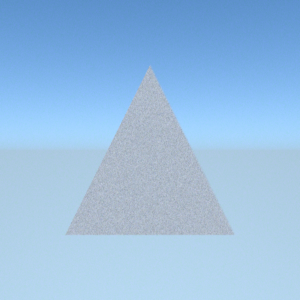
\includegraphics[width=.3\textwidth]{img/3 approach/triangle.png}\label{fig:art_triangle}}
	\hfil
	\subfloat[An example of an alytical shape: a torus aligned on Y-axis.]{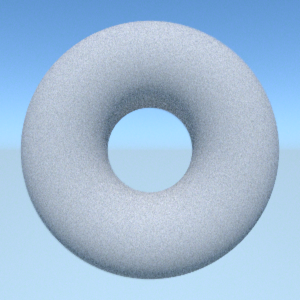
\includegraphics[width=.3\textwidth]{img/3 approach/torus.png}\label{fig:art_torus}}
	\caption{Shape types in ART.}
	\label{fig:shape_types}
\end{figure}

Although it would be convenient to initialize all shapes in ART as user defined geometries for Embree, we make the distinction between \emph{user-defined geometry} and \emph{non-user-defined geometry}.

Into the first category will fall the analytically described shapes. Triangles and quadrangles will be regarded as non user defined geometry and represented by Embree's own primitive types \texttt{RTC\_GEOMETRY\_TYPE\_TRIANGLE} and \texttt{RTC\_GEOMETRY\_TYPE\_QUAD}. This division makes sense since the rendering of these primitive types with Embree is more efficient than the rendering user defined geometries. Furthermore, all the information needed to set up these primitive types is the vertices and indices associated with the shape. They can be easily transferred from ART to Embree. 


The initialization of geometries for Embree takes place during the assembly of the scene graph from the information that has been parsed from the ARM scene file. To be precise, a particular shape is initialized for Embree when the Combined Attributes nodes and Shape nodes associated with it are created and inserted into the scene graph. After this insertion, an instance method of the \texttt{ArnEmbree} class, \texttt{initEmbreeGeometry}, is called. The shape object itself, together with the \texttt{Combined Attributes} object, and the transformation matrix, are passed as function arguments. 
\\

The \texttt{initEmbreeGeometry} function does the following:

\begin{itemize}
	\setlength\itemsep{0.05em}
	
	\item \textbf{Initialization of an \texttt{RTCGeometry}}
	\item[] To initialize a geometry for Embree, an \texttt{RTCGeometry} needs to be created. After initializing a geometry for Embree, it is committed via the function \texttt{rtcCommitGeometry}, attached to the \texttt{RTCScene} by invocation of the function \texttt{rtcAttachGeometry}, and released by calling the function \texttt{rtcReleaseGeometry}. When a particular geometry is successfully attached to the \texttt{RTCScene}, a unique identifier is assigned to it. This identifier, an unsigned integer value, is referred to as the \emph{geometry ID}. The geometry ID is stored in an instance variable of the \texttt{Shape} or \texttt{Simple Indexed Shape} class. It allows for the retrieval of the \texttt{RTCGeometry} from Embree for alteration. However, the retrieving of \texttt{RTCGeometry} variables is only possible before committing the \texttt{RTCScene}. 
	\\
	
	\item \textbf{Initialization of \texttt{GeometryData} struct and setting up the user data pointer for Embree}
	\item[] Once a shape is successfully attached to the \texttt{RTCScene}, a C struct associated with the shape is dynamically allocated and initialized. Subsequently, a user data pointer pointing to this struct is set up for Embree via the function \texttt{rtcSetGeometryUserData}. This struct, which we call \texttt{GeometryData}, stores information that is needed for calculating the intersections between a ray and a user-defined geometry in ART. It is shown in Listing \ref{lst:geometry_data}.
	\\
	
\end{itemize}

\texttt{GeometryData} structs store the geometry ID associated with the shape and issued by Embree, ART's representation of the shape in memory, a struct called  \texttt{ArTraversalState}, storing information such as the surface material of the shape, a \texttt{Combined Attributes} object, and a Boolean variable indicating if the shape is user-defined or not.

As mentioned before, user data pointer are intended to retrieve shapes in the interior of a specified callback function for ray tracing user-defined geometry with Embree. We, on the other hand, associate every shape present in a scene with such a \texttt{GeometryData} struct, even for non-user-defined geometries, solely to differentiate between these two types of shapes.

Subsequently, this struct is stored in a linked list, whose head is an instance variable of the \texttt{ArnEmbree} class. \texttt{GeometryData} structs can be extracted from this list by linear search.
 

\begin{listing} 
	\begin{lstlisting}[caption={\texttt{C} struct associated with each initialized geometry.}, label={lst:geometry_data}]
	// each geometry in the scene is associated with
	// this stuct, it is needed for embree to
	// perform user defined geometry intersection
	// calculations
	typedef struct GeometryData 
	{
		unsigned int _embreeGeomID; // geometry id of the shape
		ArNode * _shape; // ART's shape representation in memory
		ArTraversalState _traversalState; // C struct storing, e.g., surface material
		
		ArNode<ArpRayCasting> * combinedAttributes; // node used for ray casting
		BOOL _isUserGeometry; // determines if geometry is User-defined or Non-user-defined
	}
	GeometryData;
	\end{lstlisting}
\end{listing} 

\subsection{Initialization of simple indexed geometry}
Simple index geometries are initialized the following way: Inside the \texttt{initEmbreeGeometry} function, another class method with the name \texttt{initEmbreeSimpleIndexedGeometry} is called, with the shape object, the vertex set containing the vertices that describe the shape, and the transformation matrix being passed as arguments. 
\\
\\

\begin{listing} 
	\begin{lstlisting}[caption={Setting up geometry buffers for the vertices and indices of a triangle shape.}, label={lst:geometry_buffer}]
	RTCGeometry newGeometry = NULL;
	float * vertices;
	unsigned * indices;
	
	// if the shape is a triangle, 
	// create a new geometry buffer with type
	// RTC_GEOMETRY_TYPE_TRIANGLE
	if([shape isKindOfClass: [ArnTriangle class]]) 
	{
	
		newGeometry = rtcNewGeometry(device, RTC_GEOMETRY_TYPE_TRIANGLE);
		
		vertices = (float *) rtcSetNewGeometryBuffer(
													newGeometry,
													RTC_BUFFER_TYPE_VERTEX,
													0,
													RTC_FORMAT_FLOAT3,
													3*sizeof(float),
													3
													);
		
		indices = (unsigned *) rtcSetNewGeometryBuffer(
		                        newGeometry,
		                        RTC_BUFFER_TYPE_INDEX,
		                        0,
		                        RTC_FORMAT_UINT3,
		                        3*sizeof(unsigned),
		                        1
		                        );
	
	}
	\end{lstlisting}
\end{listing}


In the interior of this function, the following steps are executed:

\begin{itemize}
	\setlength\itemsep{0.05em}
	
	\item \textbf{Initialization of the \texttt{RTCGeometry}}
	\item[] Depending on whether the shape passed to it is a triangle or quadrangle, the new  variable is initialized either with the geometry type \texttt{RTC\_GEOMETRY\_TYPE\_TRIANGLE} or \texttt{RTC\_GEOMETRY\_TYPE\_QUAD}.
	\\
	
	\item \textbf{Creation of \emph{geometry buffers}}
	\item[] After this initialization is the creation and assignment of two so-called geometry buffers, one for storing the vertices and one for storing its indices that are both associated with the shape. Listing \ref{lst:geometry_buffer} shows how the function \texttt{rtcSetNewGeometryBuffer} is used to achieve that for a triangle shape.
	
	As input parameters, this function takes the \texttt{RTCGeometry} to which the geometry buffer will be linked, the buffer type, a buffer slot number, the specified format for the buffer (\texttt{RTC\_FORMAT\_FLOAT3} and \texttt{RTC\_FORMAT\_UINT3} in Listing \ref{lst:geometry_buffer}), a byte stride argument and the number of items that are about to be stored in the buffer. 
	
	The setup for the geometry buffers for quadrangles is almost identical. The only exception is that the \texttt{RTCGeometry} is initialized with the geometry type \texttt{RTC\_GEOMETRY\_TYPE\_QUAD} and that the byte stride of the vertex buffer is four instead of three.
	
	Once the geometry buffers are initialized, the vertices stored in the vertex set and indices associated with the shape are transferred to the vertex and index geometry buffers.
	\\
	
	\item \textbf{Transformation of the vertices according to the transformation matrix}
	\item[] In case the transformation matrix that was passed to the function is not \texttt{NULL}, the vertices, one by one, are transformed according to it before being transferred to the vertex buffer. Embree allows instancing of geometry, meaning that geometry in Embree can be translated, scaled, and rotated by referring to an instance stored in memory and applying this transformation to it. However, we decided to perform the transformation calculation for each vertex before transferring to the vertex geometry buffer because this is more intuitive and easier to facilitate.
	
\end{itemize}

The initialization of a triangle mesh, being parsed from a PLY file with the help of the "RPly" library \cite{rply2016}, follows the same outline described for triangles and quadrangles, although triangle meshes do not fall into the category of simple indexed shapes. The only difference is that the number of items for Embree's vertex geometry buffer is set to the number of total triangles in the mesh.

After the setup of the geometry buffers, the newly created RTCGeometry is returned from this function and assigned to the RTCGeometry, created in the \texttt{initEmbreeGeometry} function, followed by the allocation of a \texttt{GeometryData} struct and the setup of its variables. The \texttt{isUserGeometry} boolean variable is set to \texttt{false}.

\subsection{Initialization of user-defined geometry}
\label{sec:init_user}
Under this category fall any shape of ART other than triangles, quadrangles, and triangle meshes.
\\

For initializing this kind of geometry type for Embree, we do the following:

\begin{itemize}
	\setlength\itemsep{0.05em}
	
	\item \textbf{Initialization of the \texttt{RTCGeometry}}
	\item[] For user-defined geometries, the corresponding \texttt{RTCGeometry} will be initialized with Embree's primitive type \texttt{RTC\_GEOMETRY\_TYPE\_USER}.
	\\
	
	\item \textbf{Provision of a callback function for calculating the bounding box of the shape}
	\item[] We created a function called \texttt{embree\_bbox}, which Embree will call before building its internal BVHs over the scene. In the interior of the function, we calculate the bounding box of the user-defined geometry and pass it to Embree. This callback function is passed to Embree via invocation of the function \texttt{rtcSetGeometryBoundsFunction}.
	\\
	
	\item \textbf{Provision of a callback function for performing the intersection testing between a user-defined geometry and an \texttt{RTCRay}}
	\item[] For this purpose we created a function called \texttt{embree\_intersect}. We will describe this function in more detail in Section \ref{sec:embree_raycasting}. This callback function is passed to Embree via the function \texttt{rtcSetGeometryIntersectFunction}.
	\\
	
	\item \textbf{Provision of a callback function for performing the occlusion testing for a user-defined geometry}
	\item[] For ray tracing purposes, only one function for intersection calculation and occlusion testing would be necessary since both operations are performed by ray casting. However, Embree strictly expects two separate functions, each with predetermined arguments. To compensate for this, we use a strategy which was inspired by the source code of Mitsuba 2: We refractor the ray tracing functionality into a fourth function called \texttt{embree\_intersect\_geometry}, which is called from both the \texttt{embree\_intersect} and \texttt{embree\_occluded} function. 
	
\end{itemize}

Once an intersection with a bounding box enclosing a user-defined geometry is found during ray tracing, Embree will call the \texttt{embree\_intersect} function, which performs the intersection testing between the ray and the shape that is associated with that bounding box.


\section{Ray tracing with Embree in ART}
\label{sec:embree_raycasting}

Once the geometries contained in a virtual scene are initialized for Embree and Embree's internal BVH has been created, the scene can be ray cast with the help of Embree. If Embree support is enabled by provision of the \texttt{-e} flag, an instance function of the \texttt{ArnRayCaster} class with the name \texttt{getIntersectionListWithEmbree} is called, which takes an empty \texttt{ArIntersectionList} struct as an argument.

In the body of this function, an \texttt{RTCIntersectContext} is set up and a \texttt{RTCRayHit} struct is declared and updated according to the state of the \texttt{ArnRayCaster} object: The information with which the \texttt{RTCRayHit} stuct is being updated contains the orientation and direction of the ray that is stored as an instance variable of the \texttt{ArnRayCaster} object, and the ID associated to the ray. The \texttt{tfar} value of is initialized with Objective-C's \texttt{INFINITY} macro and the \texttt{geomID} field of the \texttt{RTCHit} struct is initialized with the macro \texttt{RTC\_INVALID\_GEOMETRY\_ID}. 

Embree utilizes single-precision floating-point numbers for its internal calculations, whereas ART uses double-precision floating-point numbers. To compensate for visual artifacts in the final image, we do not initialize the \texttt{tnear} value of the \texttt{RTCRay} with zero. Instead, we give it a little offset to prevent calculating an intersection between a secondary ray and the same shape that was already hit. We found the value $1e-3f$ to be reliable. A comparison of an image rendered with and without this offset is given by Figure \ref{fig:offset}.

\begin{figure}[!tbp]
	\centering
	\subfloat[Result of rendering a simple scene when the \texttt{tnear} value of the \texttt{RTCRay} is set to zero.]{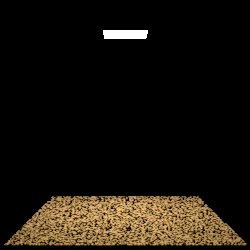
\includegraphics[width=.4\textwidth]{img/3 approach/artifact_2.png}}
	\hfil
	\subfloat[Result of rendering a simple scene when the \texttt{tnear} of the \texttt{RTCRay} is given an offset of $1e-3f$.]{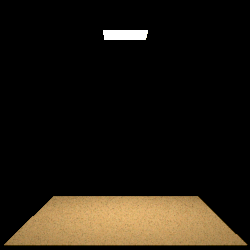
\includegraphics[width=.4\textwidth]{img/3 approach/artifact.png}}
	\caption{Artifact caused by the conversion of the hit distance of the ray from a double-precision floating-point number to a single-precision floating-point number. Due to an imprecise calculation of the intersection point, a secondary ray might intersect the same shape again.}
	\label{fig:offset}
\end{figure}

After the update of the \texttt{RTCRayHit} struct, the actual ray tracing is performed by the invocation of the \texttt{rtcIntersect1} function. Depending on whether a bounding box of a user-defined geometry or non-user-defined geometry in Embree's internal BVH was intersected by the \texttt{RTCRay}, either our custom callback function \texttt{embree\_intersect\_geometry} is called by Embree, or Embree performs the intersection testing with its proprietary functionality.

Once the overall rendering job successfully completed, a "clean-up" is performed. The \texttt{GeometryData} structs associated with the scene are released, followed by the release of the \texttt{RTCScene} via the function \texttt{rtcReleaseScene} and the release of the \texttt{RTCDevice} via \texttt{rtcReleaseDevice}. As a final step, the \texttt{ArnEmbree} object \texttt{embreeManager} itself is released.


\subsection{Intersecting user-defined geometry}
\label{subsec:instersect}

In case a bounding box of a user-defined geometry is intersected with an \texttt{RTCRay}, the callback function \texttt{embree\_intersect\_geometry} is invoked by Embree. In its interior, the \texttt{Geometry Data} struct associated with the geometry in question is retrieved via the geometry user data pointer. 

Subsequently, an empty \texttt{ArIntersectionList} struct is declared and the intersection calculation with the ray and the shape is performed via calling the \texttt{getIntersectionList} function of the \texttt{Combined Attributes} object, which takes a reference to the empty \texttt{ArIntersectionList}, as well a reference to the \texttt{ArnRayCaster} object as input.
This function will calculate the intersection points on the shape and update the \texttt{ArIntersectionList} struct accordingly. The reason why the \texttt{getIntersectionList} instance method of the \texttt{Combined Attributes} object is called, rather than the \texttt{getIntersectionList} instance method of the shape object, is that by doing so, the transformation information of the shape will be taken into account.

If no intersection was found, we return immediately from the \texttt{embree\_intersect\_geometry} function. Otherwise, we will update the \texttt{tfar} value of the \texttt{RTCRay} with the hit distance and the geometry ID of the \texttt{RTCHit} struct with the geometry ID associated with the intersected shape.
The resulting \texttt{ArIntersectionList} is then stored in a linked list.

After the invocation of the \texttt{rtcIntersect1} function in the interor of the  \texttt{getIntersectionListWithEmbree} function, the geometry ID of the \texttt{RTCHit} is evaluated. If the value of this variable remains \texttt{RTC\_INVALID\_GEOMETRY\_ID}, we conclude that no intersection was found and we return an empty \texttt{ArIntersectionList}. Otherwise, we retrieve the \texttt{RTCGeometry} that has been intersected with the geometry ID.

This \texttt{RTCGeometry} is used for the retrieval of the associated \texttt{GeometryData} struct via the user data pointer. Based on the Boolean variable \texttt{\_isUserGeometry}, we check whether the intersected shape is a user-defined geometry or a simple indexed geometry.

For the latter, we initialize the empty \texttt{ArIntersectionList}, that was passed to the \texttt{getIntersectionListWithEmbree} function "from scratch" with the updated \texttt{tfar} value of the \texttt{RTCRay}, the shape object of the \texttt{GeometryData} struct, and the \texttt{ArnRayCaster} object itself. This newly initialized \texttt{ArIntersectionList} is then returned from the \texttt{getIntersectionListWithEmbree}.

In case the intersected geometry is a user-defined geometry, the linked list, in which the calculated \texttt{ArIntersectionList}s where placed during the intersection testing, must contain at least one \texttt{ArIntersectionList} struct. We locate the \texttt{ArIntersectionList}, whose head has the minimal hit distance, by linear search. When this \texttt{ArIntersectionList} is located, we extract it from the linked list and release all other \texttt{ArIntersectionList}s stored in it. The extracted list is then assigned to the initially empty \texttt{ArIntersectionList} that was passed to the \texttt{getIntersectionListWithEmbree} function, and ART proceeds as usual until the next ray is cast.


\subsection{Resolving of encountered issues}
\label{sec:issues_user}
The following subsection outlines two major issues encountered with the approach described in the last sections. We furthermore describe how these issues can be resolved.

\subsubsection{Multi-threaded intersection testing for user-defined geometry}
As briefly mentioned in Chapter \ref{chap:art}, ART supports ray tracing with multiple threads.
Before the ray tracing procedure is initiated by ART, copies of the \texttt{ArnRayCaster} object are created for each thread. A copy of the scene graph and the KD tree is assigned to each copy of the \texttt{ArnRayCaster} object to ensure lock-free parallelism.

However, the implementation of the \texttt{embree\_intersect\_geometry} callback function for intersecting user-defined geometry is not thread safe. This is due to the \texttt{ArnRayCaster} object that needs to be passed as an argument to the \texttt{getIntersectionList} function of the \texttt{Combined Attributes} object in the interior of the \texttt{embree\_intersect\_geometry} function.

For an uncomplicated retrieval of the \texttt{ArnRayCaster} inside our custom intersection callback function, a static reference to it was originally initialized. This works fine when performing rendering jobs with only a single thread. If multiple threads are involved in the intersection computations, the procedure outlined in Subsection \ref{subsec:instersect} is prone to errors since multiple \texttt{ArnRayCaster} objects are traversing and altering a single copy of the scene graph.

To archive lock-free parallelism, we need to retrieve the "right" \texttt{ArnRayCaster} copy associated with the current thread in the interior of the intersection callback function. However, we cannot utilize the user data pointer for this since the user data pointer is associated with the scene geometry, which can be intersected by multiple rays belonging to different \texttt{ArnRayCaster} objects on different threads at the same time.

For the placement of an \texttt{ArnRayCaster} into and for the retrieval of an \texttt{ArnRayCaster} from the ray caster array, we use an identifier of the thread associated with it. We obtain the thread ID via invocation of the \texttt{gettid} function, provided with the \texttt{unistd} header file, for accessing the POSIX operating system API. The reason we chose the function \texttt{gettid} over the function \texttt{pthread\_self}, is that for $n$ cores involved for rendering, \texttt{gettid}, called from $n$ different threads, will return $n$ strictly consecutive integer values. With the help of these values we can write a fairly simple "hash" function for placing \texttt{ArnRayCaster} pointers in the ray caster array and for retrieving them from it in our intersection callback function: The index of the particualar \texttt{ArnRayCaster} pointer will be the thread ID received by the \texttt{gettid} function taken modulo with the counter variable.

During the beginning of the ray tracing procedure, a reference to the  \texttt{ArnRayCaster} object associated with the current thread is added to the ray caster array, if not already been done, retrieved in the interior of the intersection callback function in constant time, and passed to the \texttt{getIntersectionList} function of the \texttt{Combined Attributes} object. 

The head of the linked list, in which the collected intersection lists are stored, is made an instance variable of the \texttt{ArnRayCaster} class, which allows for an uncomplicated retrieval of these intersection lists outside the intersect callback function. 

\subsubsection{Intersecting infinite spheres}

A specific type of geometry supported by ART is a sphere with a huge radius. These \emph{infinite spheres} are used in a virtual scene for environment lighting.
Due to its radius, the length of the bounding box edges enclosing the infinite sphere is twice the infinite sphere's radius. 
Generally speaking, axis-aligned bounding boxes can be described by two vertices in Euclidean space, connected via the bounding box's body diagonal. In this subsection, we will refer to these vertices as \emph{upper point} and \emph{lower point}. 

In ART, all three coordinates of the upper point are set to a huge value, represented by the double value \texttt{MATH\_HUGE\_DOUBLE}, and respectively, all three coordinates of the lower point are set to the negative of that value, \texttt{- MATH\_HUGE\_DOUBLE}.

\begin{listing} 
	\begin{lstlisting}[caption={Casting of a double precision floating point number to a single precision floating point number by explicit conversion.}, label={lst:casting}]
	struct RTCBounds * bounds_o = args->bounds_o;
	
	bounds_o->lower_x = (float) boundingBox.min.c.x[0];
	bounds_o->lower_y = (float) boundingBox.min.c.x[1];
	bounds_o->lower_z = (float) boundingBox.min.c.x[2];
	
	// ...
	\end{lstlisting}
\end{listing}

As mentioned in Subsection \ref{sec:embree_raytracing}, Embree uses single-precision floating-point numbers for its internal calculations. ART, on the other hand, uses double-precision floating-point numbers. Therefore, after calculating the double values describing the bounding box, we cast them to float values via the explicit conversion operator in \texttt{C/C++} before passing them to Embree, as shown in Listing \ref{lst:casting}.  
When, during ray tracing, the \texttt{tfar} value of the \texttt{RTCRay} is set to the single-precision representation of infinity by Objective-C, the bounding box is never intersected. This is due to intersection testing being only performed in the interval $[1e-3f,\infty]$ and Objective-C's representation of infinity is "smaller" than the value \texttt{MATH\_HUGE\_DOUBLE}. The bounding box enclosing the infinite sphere is never intersected by an \texttt{RTCRay}.

Fortunately, ART provides a representation for infinity as a single-precision number as well, \texttt{MATH\_HUGE\_FLOAT}. Therefore, we can resolve this issue by checking in the \texttt{embree\_bbox} callback function whether the two vertices of the calculated bounding box have the coordinates \texttt{MATH\_HUGE\_DOUBLE} (and resp. \texttt{-MATH\_HUGE\_DOUBLE}) and updating them with the value \texttt{MATH\_HUGE\_FLOAT} (and resp. \texttt{-MATH\_HUGE\_FLOAT}). By doing so, Embree can detect intersections between an \texttt{RTCRay} and the bounding box of the infinite sphere, and the intersection with the sphere itself can be calculated.

However, we decided to exclude Embree functionality from intersection testing with this type of shape. The reason for this lies in the further reduction of the number of unnecessary intersection calculations. If an intersection point on the infinite sphere is occluded by other scene geometry, we can ignore it. Therefore we only calculate the intersection between a ray and the infinite sphere if the ray did not intersect other scene geometry.

\subsubsection{Consecutive intersection of user-defined and non-user-defined geometry}

With the approach described in Section \ref{subsec:instersect}, an issue arises when ray tracing virtual scenes which contain both user-defined and non-user-defined geometry. In such scenes, a cast ray could consecutively intersect a non-user-defined geometry and a user-defined geometry. To give an example, this is the case for the virtual scene displayed in \ref{fig:no_bunny}. This scene is composed of a quadrangle serving as the ground plane, the Stanford Bunny triangle mesh, which was provided by the Stanford 3D Scanning Repository \cite{plyRepo}, and an infinite sphere for environment lighting.

Given a ray that first intersects the PLY mesh and subsequently the infinite sphere, we noticed that through the invocation of the \texttt{rtcIntersect1} function, Embree internally calculates the intersections between the ray and the triangle mesh first and then calls the \texttt{embree\_intersect} callback function to calculate the intersection point with the infinite sphere.


\begin{figure}[!tbp]
	\centering
	\subfloat[Scene rendered with Native ART.]{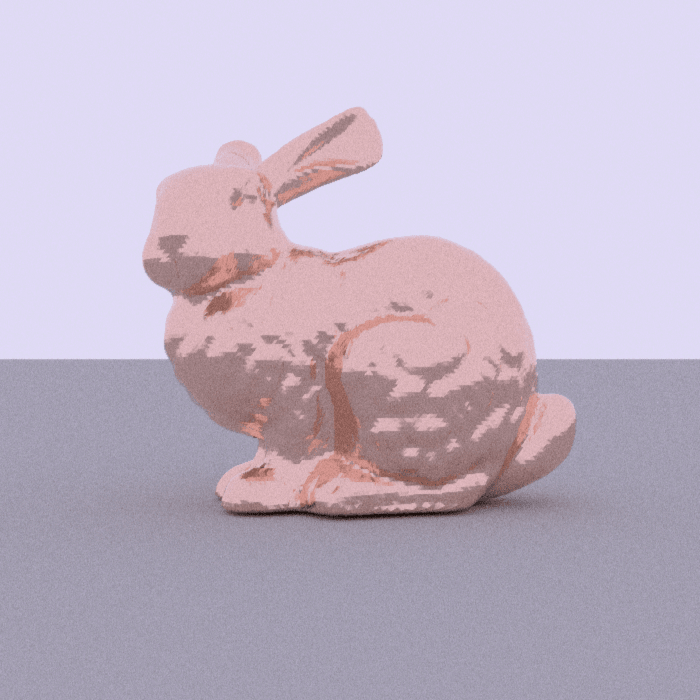
\includegraphics[width=.4\textwidth]{img/3 approach/bunnyNormal.png}} 
	\hfil
	\subfloat[Scene rendered with the approach outlined in Section \ref{sec:embree_raycasting}]{
\includegraphics[width=.4\textwidth]{img/3 approach/bunnyError.png} \label{fig:no_bunny_close}}
	\caption{Rendered images of a scene containing a non-user-defined triangle mesh and quadrangle, and a user-defined user-defined infinite sphere, illuminating the rest of the sphere.}
	\label{fig:no_bunny}
\end{figure}


The problem, which arises here, is that the values of the \texttt{RTCRayHit} struct, e.g., the \texttt{tfar} value of the \texttt{RTCRay}, are updated with information corresponding to the intersection with the triangle mesh first. Afterward, the user-defined infinite sphere is intersected, and the intersection calculation is performed by our custom function \texttt{embree\_intersect\_geometry} function. In the interior, we overwrite the values of the \texttt{RTCRayHit} struct that has been previously calculated while the triangle mesh was intersected. Therefore, the information regarding the intersections between the \texttt{RTCRay} and the triangle mesh is lost, and only the \texttt{ArIntersectionList} storing the intersections with the infinite sphere is present in the linked list. A result of this behavior can be seen in Figure \ref{fig:no_bunny_close}.

To resolve this issue, we make use of a slight hack: In the interior of the \texttt{embree\_intersect\_geometry} callback function, before performing the actual intersection calculation between a ray and a user-defined geometry, we check whether the value of the geometry ID of the \texttt{RTCHit} struct remains being set to \texttt{RTC\_INVALID\_GEOMETRY\_ID}. If this is not the case, and if the head of the linked list storing the collected intersections is not \texttt{NULL}, we conclude that an intersection with a non-user-defined geometry must have already been calculated. We assume that is intersection already obtains the closest distance to the ray origin. With the help of the geometry ID, we retrieve the associated \texttt{GeometryData} struct for the geometry in question from the linked list storing all the \texttt{GeometryData} structs linked to the scene geometry. With the information stored in this \texttt{GeometryData} struct, we initialize a \texttt{ArIntersectionList} "from scratch" and add it to the linked list storing the collected intersections.

With this approach, all the scenes on which our implementation was tested (which will be introduced in Chapter \ref{chap:results}) could be rendered without further problems.


\section{Rendering CSG with Embree}
\label{sec:embree_csg}

Unfortunately, Embree does not support rendering of constructive solid geometry direct. However, this does not mean that ray tracing CSG with Embree is completely impossible \todo{maybe reformulate}. The following section outlines three different approaches for ray tracing virtual scenes containing constructive solid geometry with the help of Embree. We then describe our final implementation of the CSG operators in ART as a combination of these approaches.

Since Embree is an open-source framework, one could consider rigging Embree itself for suitable CSG rendering. Nevertheless, we refrained from such an undertaking due to two reasons: On one hand, it is possible that the altering of the Embree framework would exceed the scope of this thesis. On the other hand, we want our integration to be compatible with the original Embree framework in its current and future versions. 

We therefore consider Embree as a "black box" for which we provide information such as a ray origin and direction, and receive in turn information such as the hit distance an the surface normal at the hit point.


\subsection{Evaluation of collected intersections according to the scene graph}
\label{subsec:apprach1}

In the past, an attempt for the implementation of CSG rendering with Embree was conducted by Karaffová and described in her master thesis \cite{karaffova2016}. Her approach consists in the collection of intersections between the scene geometry and a ray that are calculated by Embree, and their subsequent evaluation and arrangement according to a provided CSG tree. The difference between this work and the work of this thesis is that instead of integrating Embree into a target application that supports CSG rendering,  \todo{later}.
With the approach outlined in this subsection, we adapt the procedures described in \cite{karaffova2016} for ART, which serves as the target application. 

For the moment, we will not consider the constructive solid geometry that is (at least partially) constructed from simple indexed shapes. An explanation for this will follow later.

The intersections between a ray and user defined scene geometry can be collected via storing the corresponding \texttt{ArIntersectionLists} in a linked list as described in subsection \ref{subsec:instersect}. One advantage of maintaining such a "list of intersection lists" as opposed to the merging of the various intersection lists into one large list, is that due to the fact that each intersection list is associated with an individual geometry, we can separate the lists according to their shapes. This is convenient since ART provides functions for evaluating two given \texttt{ArIntersectionList} structs according to the binary operators \texttt{OR}, \texttt{AND} and \texttt{SUB} (the name of these functions are \texttt{arintersectionlist\_or}, \texttt{arintersectionlist\_and} and \texttt{arintersectionlist\_sub}, each taking two \texttt{ArIntersectionList} structs as input and returning a merged \texttt{ArIntersectionList} struct).

For our approach on the implementation of CSG operations with Embree, 

\begin{listing} 
	\begin{lstlisting}[caption={Updated \texttt{GeometryData} struct for CSG rendering.}, label={lst:geometry_data_update1}]
	// each geometry in the scene is associated with
	// this stuct, it is needed for embree to
	// perform user defined geometry intersection
	// calculations
	typedef struct GeometryData 
	{
		unsigned int _embreeGeomID; // geometry id of the shape
		ArNode * _shape; // ART's shape representation in memory
		ArTraversalState _traversalState; // state of the RayCaster
		
		ArNode<ArpRayCasting> * combinedAttributes; // node used for ray casting
		BOOL _isUserGeometry; // determines if geometry is User-defined or Non-user-defined
		BOOL _isCSGPrimitive; // determines if geometry is a part of a CSG
		
		ArNode<ArpRayCasting> * topmostCSGNode; // reference to the topmost CSG node 
	}
	GeometryData;
	\end{lstlisting}
\end{listing}

The sub tree of the scene graph rooted at such a topmost CSG node will serve as the CSG tree according to which the collected intersection will be evaluated and rearranged.


Once a rendering pass with Embree has finished, we retrieve the associated \texttt{GeometryData} struct of the most recently intersected geometry. If the geometry in question is not a part of a CSG, we proceed as usual. Otherwise, we evaluate the collected intersections stored in the linked list according to the sub tree rooted at the top most CSG node. 

During the evaluation, the sub tree rooted at the topmost CSG node is traversed, the intersections with the two geometries represented by the children of the node are calculated and then re-arranged according to the binary operator associated with the topmost CSG node. Due to the reason that some intersections have already been calculated previously by Embree, we first check whether an \texttt{ArIntersectionList} struct associated with the underlying geometry is already present in the linked list. If this is the case, the corresponding \texttt{ArIntersectionList} structs are located in the linked list by linear search, extracted from it, later evaluated according to the CSG operation and finally, the resulting \texttt{ArIntersectionList} is placed into the linked list.


Subsequently, when the nodes representing the individual geometric primitives are added as leaves to the sub tree rooted at the topmost CSG node, and the flag was activated, a boolean indicating that the shape in question is a primitive of a CSG is stored in the \texttt{GeometryData} struct. Furthermore, the reference to the top most CSG node is transferred from the instance variable of the \texttt{ArnEmbree} class to the \texttt{GeometryData} struct. The updated \texttt{GeometryData} struct is shown in Listing \ref{lst:geometry_data_update1}.


Since ART supports instancing of geometry, we use the \texttt{Combined Attributes} node as a unique identifier for the retrieval of the \texttt{ArIntersectionList} associated with the intersected geometry from the various \texttt{ArIntersectionList} structs that are stored in the linked list.
Therefore we add a reference to the \texttt{Combined Attributes} object of a shape to the struct that is defining the node for the intersection collection linked list. This struct is shown in Listing 

After the evaluation, the intersection list, whose head intersection has the shortest distance to the ray origin is extracted from the linked list, and the ray tracing procedure is carried on as usual.

This approach is error prone to non user defined geometries due to the issues related of the consecutive intersection calculations on user defined and non user defined geometry, described in Subsection \ref{sec:issues_user} \todo{definitely rephrase}. However, this issue can be resolved by the instantiation of simple indexed geometry as user defined geometry.

The results of \cite{karaffova2016} showed that


\subsection{Initializing the complete CSG as user-defined geometry}
\label{subsec:apprach2}

The increased render times that resulted from the previous approach served as a motivation for the development of superior procedures for ray tracing CSG with Embree. 

The core idea of the approach outlined in this Subsection lies in the initialization of the whole constructive solid geometry as a user defined geometry as opposed to its geometric primitives. If a bounding box enclosing a particular CSG would be stored in Embree's internal BVHs, and if one such bounding box is intersected by an \texttt{RTCRay}, the intersection calculation of the individual primitives would be carried on by ART's internal ray acceleration data structures. Since Embree does not directly support the ray tracing of constructive solid geometry, and we do not want to alter the Embree framework itself for reasons mentioned earlier, this undertaking seems like a satisfactory compromise between ART and Embree.

For our new approach, we define the \emph{topmost CSG node} in the scene graph as the root node of the subgraph, representing the CSG in question. The geometric primitives represented by the leaf nodes of this subgraph construct the entire CSG. For example, when considering the scene graph the CSG shown in Figure \ref{fig:csg_or}, which itself is shown in Figure \ref{fig:scene_graph}, the topmost CSG node of the CSG would be the "\texttt{OR}-node", having two instances of the singleton sphere (indicated through the "\texttt{Bounding Box}-" and "\texttt{Combined Attribute}-nodes") for its children.

When during the initial assembly of ART's internal scene graph such a topmost CSG node is encountered, a class method of the \texttt{ArnEmbree} class, \texttt{initEmbreeCSGGeometry}, is called, which initialized a new \texttt{RTCGeometry} of type \texttt{RTC\_GEOMETRY\_TYPE\_USER}. 
Callback functions for intersection and occlusion testing, as well as for calculating the bounding box of the CSG are provided as outlined in Subsection \ref{sec:init_user}. 


\begin{listing} 
	\begin{lstlisting}[caption={Updated \texttt{GeometryData} struct for CSG rendering.}, label={lst:geometry_data_final}]
	// each geometry in the scene is associated with
	// this stuct, it is needed for embree to
	// perform user defined geometry intersection
	// calculations
	typedef struct GeometryData 
	{
		unsigned int _embreeGeomID; // geometry id of the shape
		ArNode * _shape; // ART's shape representation in memory
		ArTraversalState _traversalState; // state of the RayCaster
		
		ArNode<ArpRayCasting> * _combinedAttributes_or_csg_node; // node used for ray casting
		BOOL _isUserGeometry; // determines if geometry is User-defined or Non-user-defined
	}
	GeometryData;
	\end{lstlisting}
\end{listing}

Subsequently, a \texttt{GeometryData} struct is created. The struct itself was slightly adapted for CSG rendering. As can be seen in Listing \ref{lst:geometry_data_final}, we renamed the variable storing a reference to the \texttt{Combined Attribute} node to \texttt{\_combinedAttributes\_or\_csg\_node}. Both the \texttt{Combined Attributes} node object and the topmost CSG node derive from the \texttt{ArNode} base class, and through the implementation of the \texttt{ArpRayCasting} protocol, they provide functionality for calculating the bounding box enclosing their children and performing intersection testing.
When a CSG is getting initialized as a user defined geometry, a reference to the topmost CSG node is assigned to the
\texttt{\_combinedAttributes\_or\_csg\_node} variable.

A flag gets activated after a successful initialization of a constructive solid geometry during the scene graph assembly. When the traversal of a scene graph continues to the leaf nodes representing the geometric primitives of the CSG, they do not get initialized as user defined geometry when this flag is activated.

During the intersection calculation by the \texttt{embree\_intersect} callback function during the rendering, the \texttt{getIntersectionList} function of the \texttt{\_combinedAttributes\_or\_csg\_node} object is called. Depending of this node being a \texttt{Combined Attributes} node or a topmost CSG node, the rendering procedure diverges: For a \texttt{Combined Attributes} node, the intersections are calculated directly on the shape, taking transformation information into account. For a topmost CSG node, the intersections with the underlying primitives are calculated by traversing the sub scene graph rooted at that node, as outlined in Section \ref{sec:art_raytracing}. 

With this approach, scenes containing constructive solid geometries can be successfully rendered and the performance of the ray tracing process increased compared to the previous approach.  A detailed comparison of these two approaches can be found in Chapter \ref{chap:results}. Furthermore, the artifacts that result from rendering a scene in native ART by traversal of the "original scene graph", as described in Subsection \ref{sec:art_raytracing} are not present in images rendered with this approach, although the same "original scene graph" is partially traversed.

However, there exists some limitations with this approach. One issue was encountered when rendering a specific CSG scene: The Villa Rotonda scene, shown in Figure \ref{fig:rotonda}. Figure \ref{fig:rotonda_embree} shows the final image, rendered by the described approach. The figure shows the villa with its roof missing. At this point, we have to admit that we were not able to resolve this issue \todo{rephrase?}. However, due to the fact that rendering the scene with native ART by traversal of the original scene graph had the same outcome (apart from the visible noise), and due to the fact that we did not encounter this issue with other scene files containing CSG, we assume that this is a bug of the target platform ART. \todo{rephrase}

\todo{or infsphere}

\todo{triangle csg}





\begin{figure}
	\centering
	\subfloat[Villa Rotonda scene rendered with native ART by traversing the interlan KD tree.]{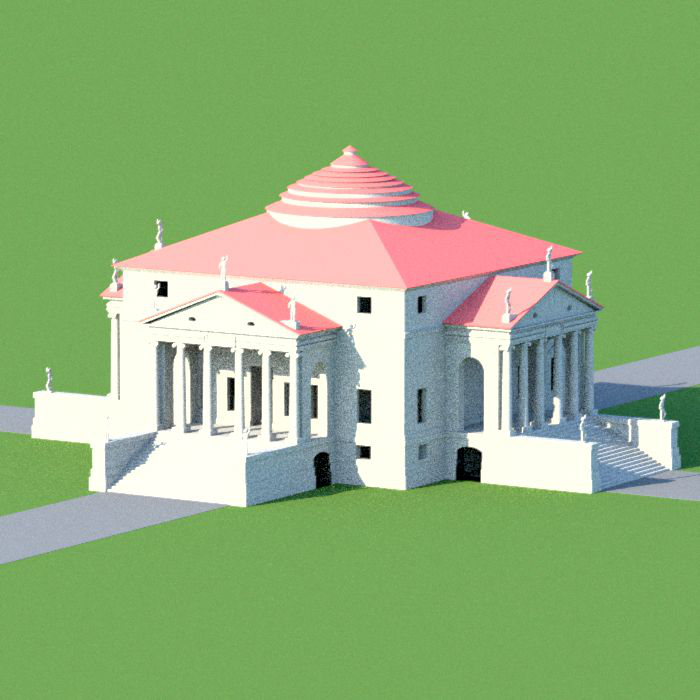
\includegraphics[width=.3\textwidth]{img/3 approach/villaRotondaNormal.png}\label{fig:rotonda_normal}}
	\hfill
	\subfloat[Villa Rotonda scene rendered with Embree.]{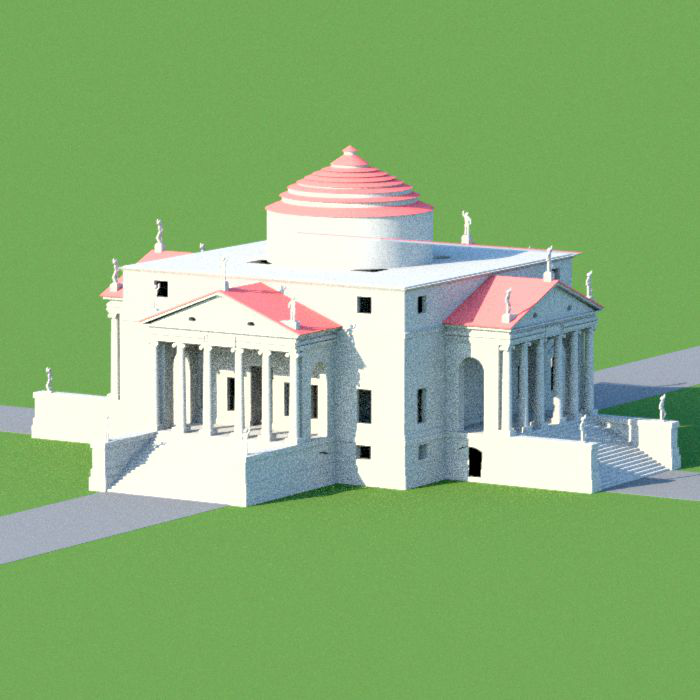
\includegraphics[width=.3\textwidth]{img/3 approach/villaRotondaEmbree.png}\label{fig:rotonda_embree}}
	\hfill
	\subfloat[Villa Rotonda scene rendered with native ART by traversing the original scene graph.]{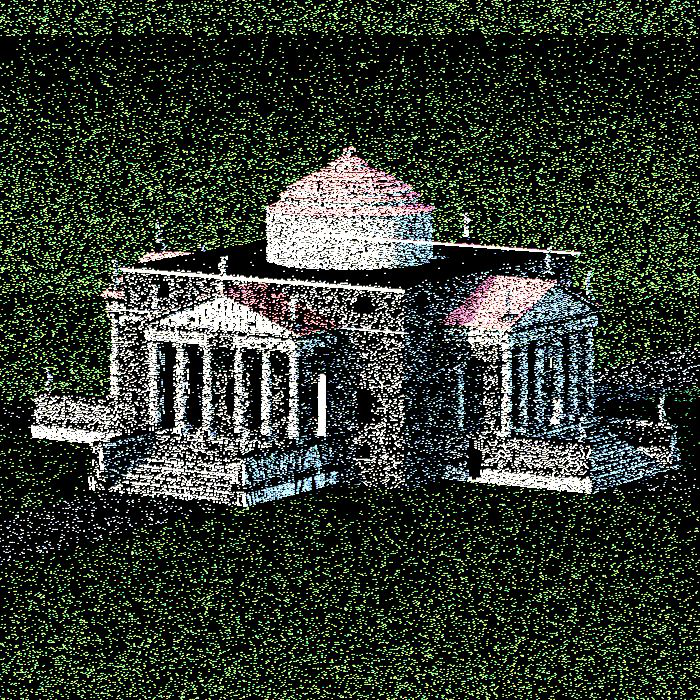
\includegraphics[width=.3\textwidth]{img/3 approach/villaRotondaOrgScenegraph.png}\label{fig:rotonda_orgscenegraph}}
	\caption{Artifact in the Villa Rotonda scene: The villa is missing its roof.}
	\label{fig:rotonda}
\end{figure}


\subsection{Creation of KD trees for constructive solid geometries}
\label{subsec:apprach3}
bla blub